\chapter{Multiple Evolutionary Origins of Ubiquitous Cu2+\newline and Zn2+ Binding in the S100 Protein Family}


\section{Author Contributions}
Lucas Wheeler and Michael Harms conceptualized the study and designed experiments. Michael Harms acquired funding for the study. Lucas Wheeler and Micah Donor performed experiments and analyzed experimental data. Michael Harms and James Prell administered the project. Michael Harms conducted phylogenetic analyses. Lucas Wheeler and Michael Harms wrote and edited the manuscript.

\section{Abstract}

The S100 proteins are a large family of signaling proteins that play critical roles in biology and disease. Many S100 proteins bind Zn$^{2+}$, Cu$^{2+}$, and/or Mn$^{2+}$ as part of their biological functions; however, the evolutionary origins of binding remain obscure. One key question is whether divalent transition metal binding is ancestral, or instead arose independently on multiple lineages. To tackle this question, we combined phylogenetics with biophysical characterization of modern S100 proteins. We demonstrate an earlier origin for established S100 subfamilies than previously believed, and reveal that transition metal binding is widely distributed across the tree. Using isothermal titration calorimetry, we found that Cu$^{2+}$ and Zn$^{2+}$ binding are common features of the family: the full breadth of human S100 paralogs---as well as two early-branching S100 proteins found in the tunicate \textit{Oikopleura dioica}---bind these metals with $\mu$M affinity and stoichiometries ranging from 1:1 to 3:1 (metal:protein). While binding is consistent across the tree, structural responses to binding are quite variable. Further, mutational analysis and structural modeling revealed that transition metal binding occurs at different sites in different S100 proteins. This is consistent with multiple origins of transition metal binding over the evolution of this protein family. Our work reveals an evolutionary pattern in which the overall phenotype of binding is a constant feature of S100 proteins, even while the site and mechanism of binding is evolutionarily labile.

\section{Introduction}

The S100 protein family is an important group of calcium binding proteins
found in vertebrates \cite{donato_functions_2013,zimmer_evolution_2013}.
Humans possess 27 family members that play diverse functional roles
in inflammation \cite{wolf_chemotactic_2008,leclerc_binding_2009,sorci_danger_2011},
cell proliferation \cite{shaw_s100b-rage-mediated_2003,klingelhofer_epidermal_2009,wang_s100a14_2015},
and innate immunity \cite{yang_s100a12_2007,damo_molecular_2013,zackular_nutritional_2015}.
S100 proteins are particularly prominent in inflammatory diseases
and cancers, where they are used both as clinical markers and drug
targets \cite{marenholz_s100_2004,sedaghat_s100_2008,donato_rage:_2007,west_s100a7_2010,averill_s100a9_2011,riuzzi_s100b_2011,boye_s100a4_2010,yamaoka_gene_2013,gross_joining_2013,bresnick_s100_2015}.
S100 proteins are found only in chordates and are highly diverged
from other calcium binding proteins \cite{zimmer_evolution_2013,marenholz_s100_2004}.

Most S100 proteins share a common homodimeric structure in which $\sim$10
kDa monomers come together to form a compact $\alpha$-helical fold
(Fig 4A). Each monomer binds two Ca$^{2+}$ ions in conserved calcium
binding motifs, inducing a conformational change that exposes a hydrophobic
surface \cite{bertini_solution_2012,santamaria-kisiel_calcium-dependent_2006,rustandi_ca2+-dependent_1998}.
This surface can then interact with and modulate the activity of downstream
target proteins \cite{zimmer_molecular_2003,zimmer_calcium-dependent_2010}.

In addition to Ca$^{2+}$, many S100 proteins interact with divalent
transition metals such as Zn$^{2+}$, Cu$^{2+}$, or Mn$^{2+}$ as
part of their biological functions \cite{moroz_role_2010,gilston_binding_2016}.
Such functions include metal transport \cite{sivaraja_copper_2006},
modulation of signaling \cite{heierhorst_interaction_1997}, and antimicrobial
activity \cite{damo_molecular_2013}. Their transition metal binding
constants tend to be $\sim$$\mu$M, consistent with their roles in
metal transport and metal-dependent signaling \cite{ohalloran_metallochaperones_2000,maret_zinc_2013}.
Despite the importance played by these metals, transition metal binding
has not been studied systematically across the family \cite{moroz_role_2010,gilston_binding_2016}.
While one key transition metal site\textemdash at the dimer interface\textemdash has
been studied extensively (Fig 4B), the transition metal binding capacity
of many S100 proteins remains unknown. For many others, there are
conflicting reports about the binding affinities, sites, and stoichiometries
for binding to divalent transition metals \cite{moroz_role_2010,gilston_binding_2016}.

\begin{figure}
\centering
	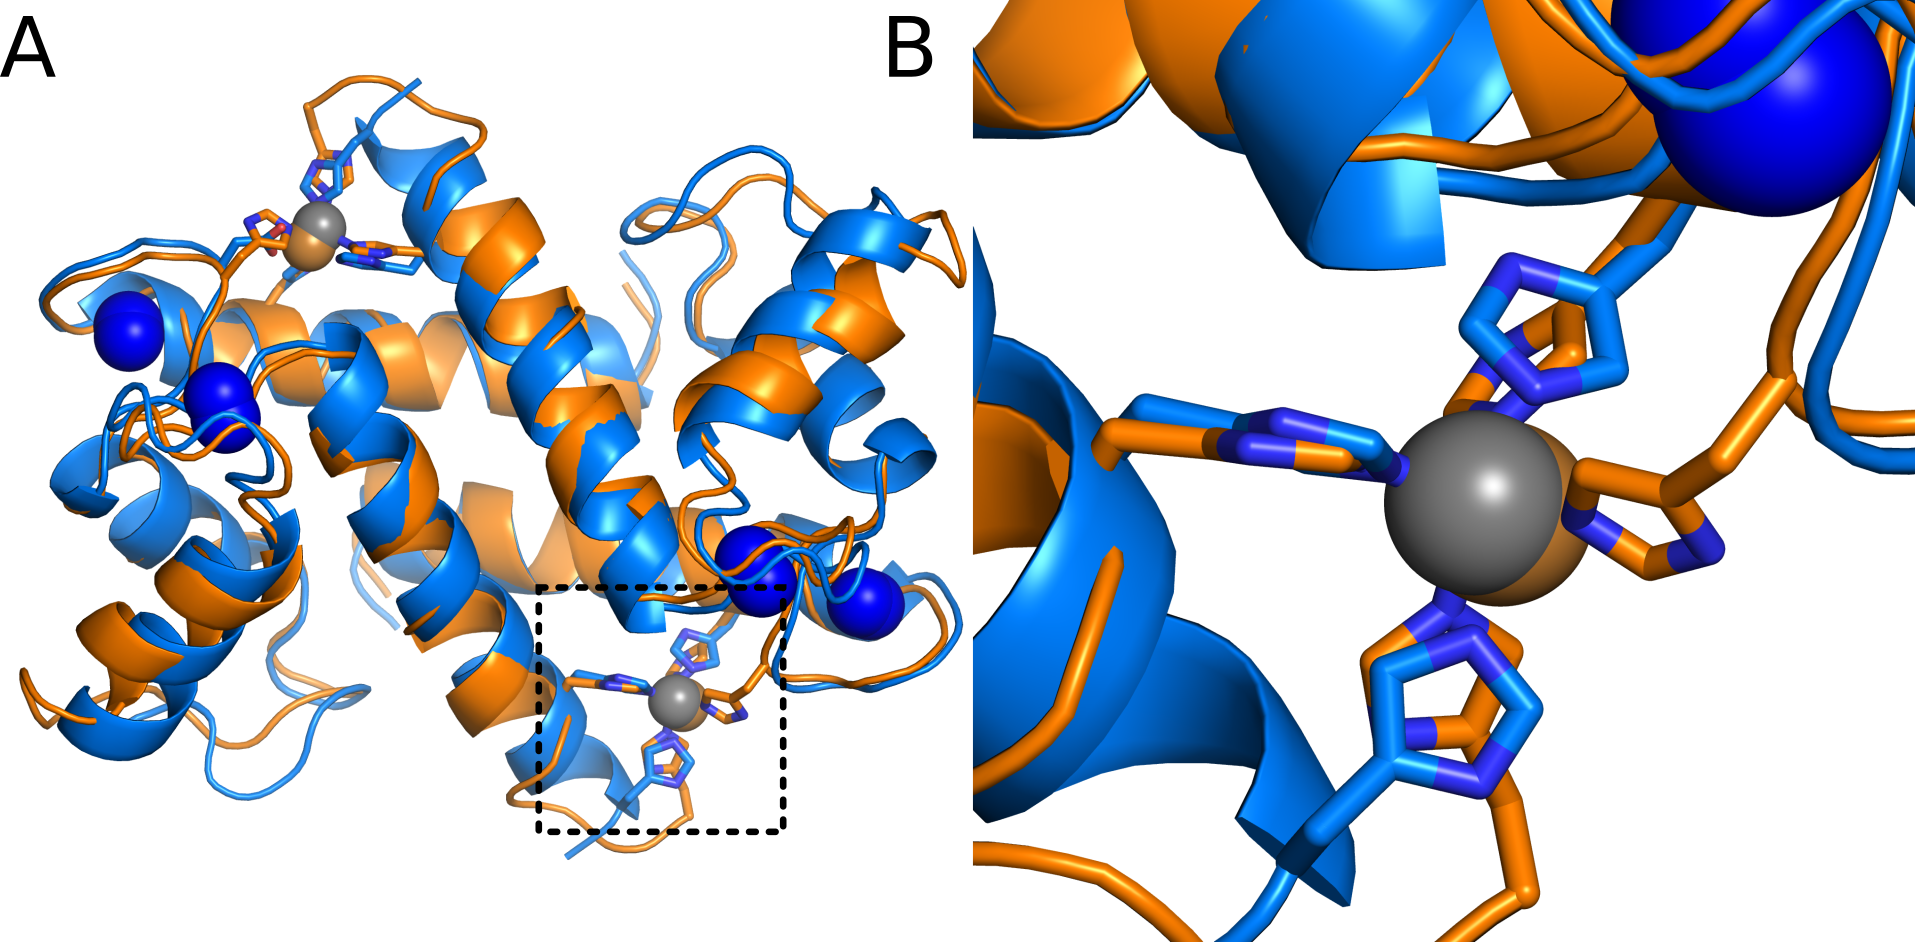
\includegraphics{ch3-fig1.png} 
\caption[Transition metal binding occurs at a common site in diverse S100s]{Transition metal binding occurs at a common site in diverse S100 proteins. Overlay of the crystal structures of S100B (orange, PDB 3CZT) and S100A12 (blue, PDB 1ODB) bound to Ca2+ and transition metals. Ions are shown as colored spheres: Ca$^{2+}$ (blue), Zn$^{2+}$ (gray) and Cu$^{2+}$ (copper). Residues ligating the transition metals are are shown as sticks. Boxed region is shown in detail in panel B.\label{samplefigure}}	
\end{figure}

Evolutionary history provides a powerful lens through which to understand
this metal binding diversity and its accompanying functional diversity.
Understanding when a feature evolved in the family, and thus which
homologs might share the feature, helps translate observations for
one family member into predictions about other family members. One
key question is whether transition metal binding is a shared ancestral
feature, or whether it has been acquired independently on multiple
lineages. Although all five crystal structures of S100 proteins bound
to transition metals have similar binding sites (Fig 4B), experimental
evidence suggests that other S100s bind to divalent transition metals
at a different site than the one identified crystallographically \cite{arnesano_structural_2005,koch_implications_2007},
consistent with at least one more acquisition of transition metal
binding.

A well-supported phylogeny of the S100 protein family would allow
observations of transition metal binding to be mapped as evolutionary
characters, thereby allowing inferences about the evolutionary history
of the character. Several phylogenies have been published \cite{zimmer_evolution_2013,marenholz_s100_2004,ravasi_probing_2004,kraemer_structural_2008,shang_chromosomal_2008},
however, these trees are not fully consonant with one another, making
interpretation difficult. Previous analyses were limited by the number
of S100 sequences available, particularly from early-branching vertebrate
species. Further, all but one \cite{kraemer_structural_2008} relied
on distance-based phylogenetic methods. Increased taxonomic sampling,
combined with more advanced phylogenetic methods, will provide a much
clearer picture of S100 evolution.

We therefore set out to understand the evolution of transition metal
binding in this family through a combination of phylogenetic analysis
and biochemical characterization of select human paralogs. Further,
to establish the ancient features of the family, we performed the
first-ever biochemical characterization of two early-diverging S100
proteins from the tunicate \textit{Oikopleura dioica}. Our work sheds
light on the evolutionary process that gave the diversity of modern
S100 proteins, as well as revealing the broad-brush evolution of the
transition-metal binding phenotype of this important protein family.


\section{Results}

\subsection{The S100 family arose in the ancestor of Olfactores}

Our first goal was to establish the taxonomic distribution of the
S100 family. We began with an iterative BLAST approach. We used the
full set of 27 human S100 family members (S1 Table in supplementary directory) as a starting
point for PSI-BLAST against the NCBI non-redundant protein database.
In addition to identifying thousands of S100 sequences, this protocol
picked up non-S100 calcium binding proteins such as calmodulin and
troponin, indicating that we had saturated S100 proteins in the database.
We filtered our hits by reverse BLAST. All S100 hits were within vertebrates,
with the exception of four hits from the tunicate \textit{Oikopleura
dioica}. To further support the taxonomic distribution of the S100s,
we then used BLAST to search directly in the genomes and transcriptomes
from representative tunicates, cephalochordates, hemichordates, and
echinoderms. Only a transcriptome from the tunicate Molgula tectiform
yielded a further S100 hit. We also queried the HMMER database, but
found no new S100 family members. The presence of S100 proteins in
tunicates and vertebrates (Olfactores), but not other chordates, suggests
that the first S100 arose in the last common ancestor of tunicates
and vertebrates, $\sim$700 million years ago \cite{hedges_molecular_2006}.
These results are consistent with previous studies that noted the
relative youth of the S100 family\cite{zimmer_evolution_2013,marenholz_s100_2004,kraemer_structural_2008,shang_chromosomal_2008}.


\subsection{Model-based phylogenetic approaches reveal well-supported clades}

We next constructed a phylogenetic tree, using sequences drawn from
across Olfactores. Phylogenetic analyses of this family are challenging
as it is large and diverse. For example, the average sequence identity
of the 27 human family members is 29.5\%, with the most divergent
pair (A3 and A14) only 13.2\% identical. Further, the small size of
these proteins ($\sim$100 amino acids) means they have few evolutionary
characters and, thus, relatively weak phylogenetic signal. Finally,
many S100 paralogs exhibit highly specific tissue distributions, meaning
that transcriptomes can provide very incomplete pictures of the S100
complement of a given organism.

To construct a tree despite these difficulties, we assembled a high-quality
dataset of 564 sequences, from 52 species, through targeted searches
of key genome/transcriptome/proteome databases (S2 Table, S1 Spreadsheet in supplementary directory).
In an effort to bracket the class-level evolutionary origin of each
S100 ortholog\textemdash despite incomplete sequence data and possible
differential loss along each lineage\textemdash we included multiple
species within each class: two Tunicata (one Ascidiacea, one Appendicularia),
two Agnathan (jawless fishes), seven Chondrichthyans (cartilaginous
fishes), eight Actinopterygii (ray-finned fishes), three Sarcopterygii
(lobe-finned fishes), seven Amphibians, fourteen Sauropsids (birds
and reptiles), and seven Mammals (two monotremes, two therians, and
three eutherians). We generated a 133 character alignment from these
sequences (Fig 24 in supplement and S2 Fig in supplementary directory, S1 Alignment) and used this for model-based
phylogenetics.

We used both maximum likelihood (ML) and Bayesian approaches to construct
phylogenetic trees for the family (Fig 5, S1 Tree and S2 Tree in supplementary directory, Fig 25 in supplement
). Both approaches resolved well-supported clades containing each
of the human seed paralogs. This allowed us to assign the orthology,
relative to the human proteins, for 500 of the 564 sequences in our
data set (S1 Spreadsheet in supplementary directory). In addition, the ML and Bayesian approaches
revealed a set of consonant clades: A2/A3/A4; A5/A6; the calgranulins
(A7/A8/A9/A12); A13/A14; and the so-called \textquotedblleft fused\textquotedblright{}
family (cornulin/ trichohyalin/repetin/hornerin/filaggrin) (Fig 5
and Fig 25 in supplement). In the Bayesian consensus tree, no further relationships
could be resolved. Several other clades were resolved in the ML tree
(Fig 5); A2/A3/A4 groups with A4/A5; A10 with A11; and A13/A14 groups
with A16. In both trees, the sum of the branch lengths was extremely
long, reflecting the high diversity of the family.

\begin{figure}
\centering
	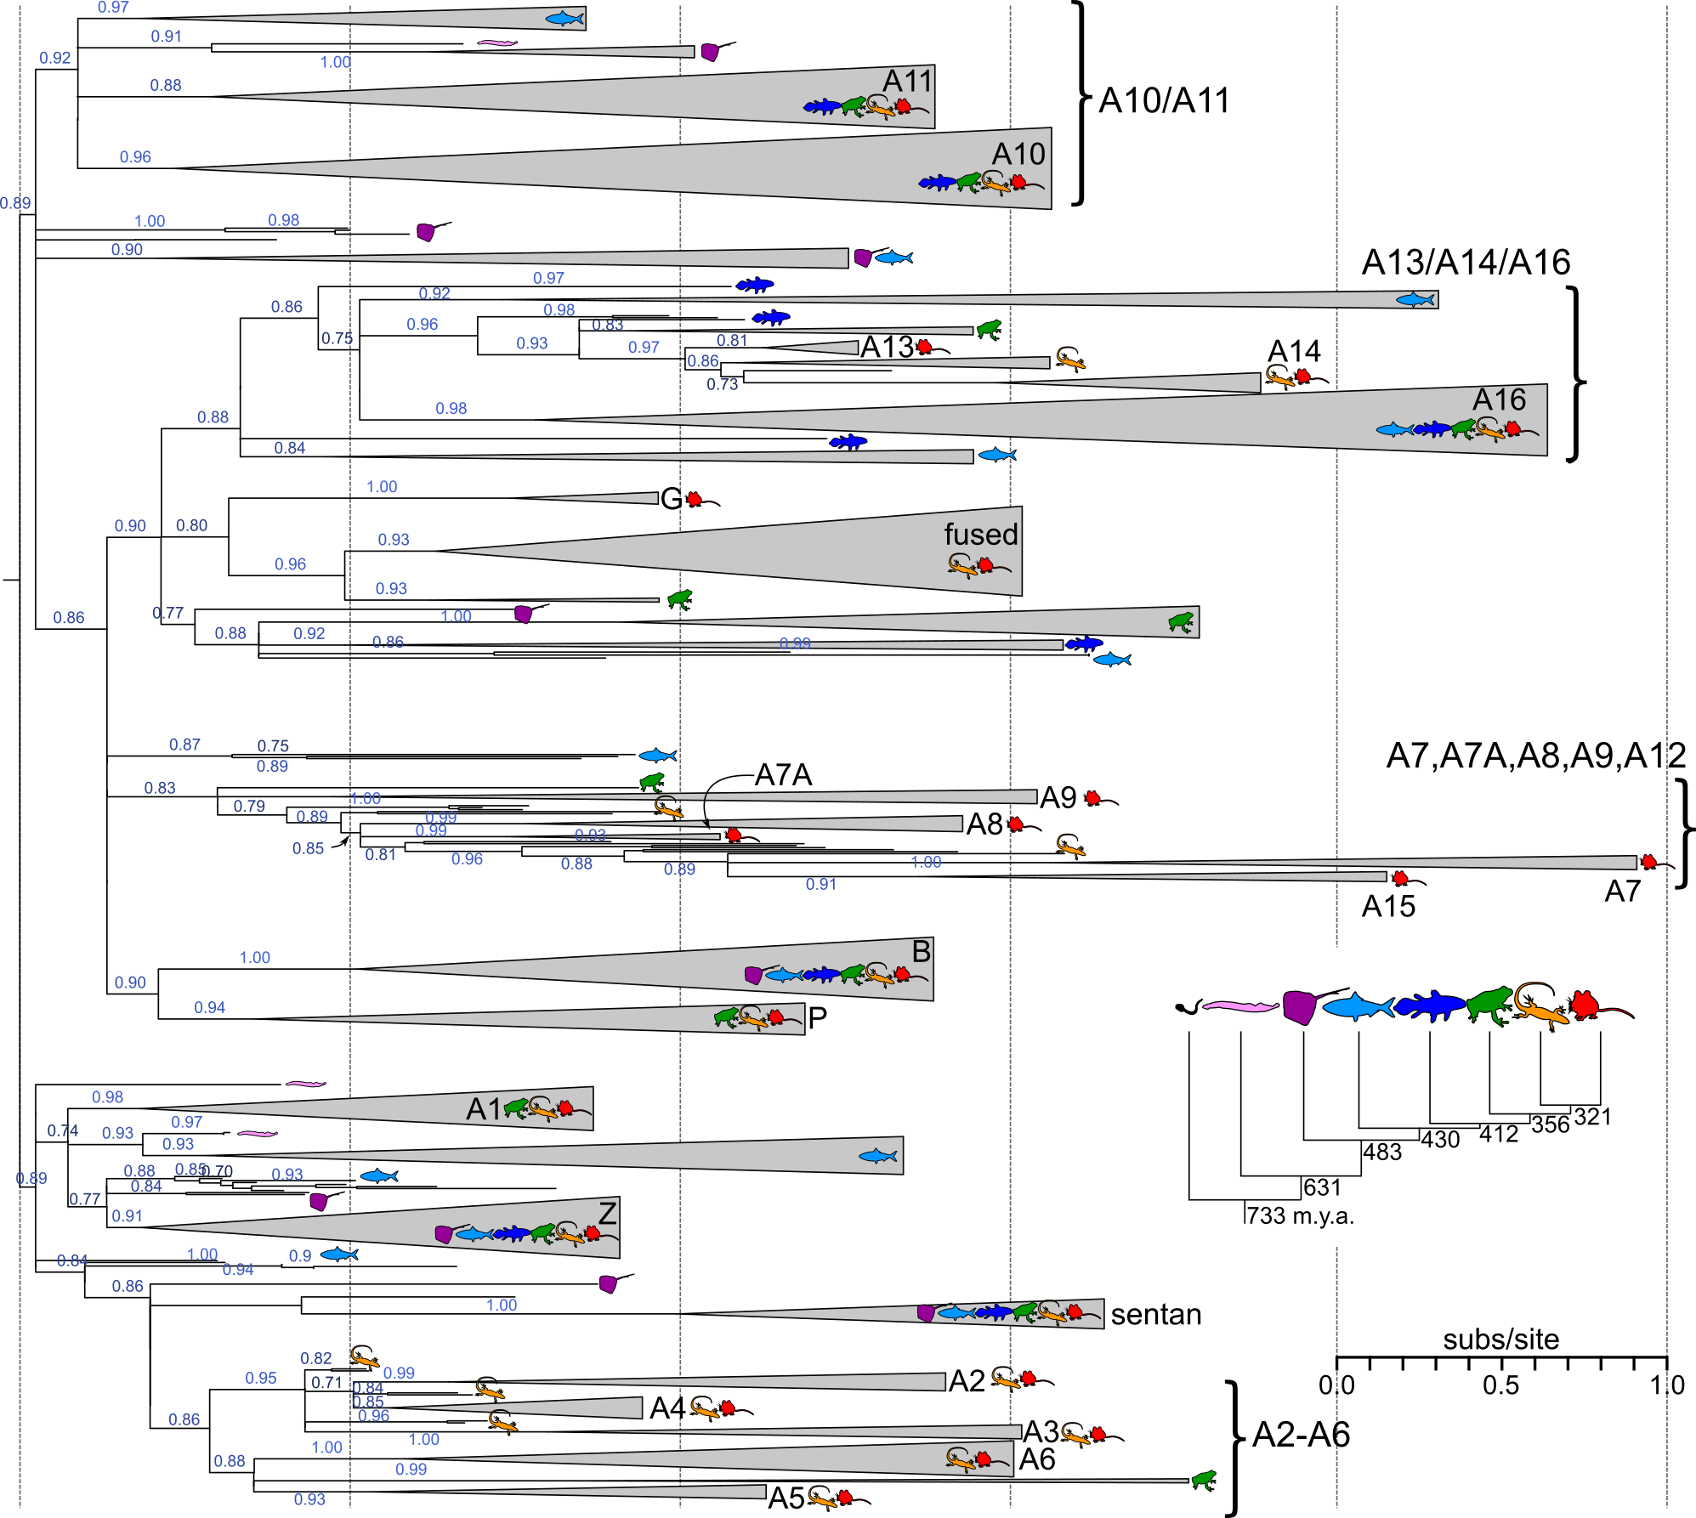
\includegraphics{ch3-fig2-smaller.png} 
\caption[Model-based phylogenetics reveal several S100 subfamilies]{Model-based phylogenetics reveal several S100 subfamilies.
Maximum likelihood phylogeny of 564 S100 proteins drawn from 52 Olfactores species. Wedges are collapsed clades of shared orthologs, with wedge height denoting number of included taxa and wedge length denoting longest branch length with the clade. Support values are SH-supports, derived from an approximate likelihood ratio test. Rooting is arbitrary, but roughly balances the distribution of jawless fishes across the ancestral node. Icons indicate taxonomic classes represented within each clade: tunicates (black), jawless fishes (pink), cartilaginous fishes (purple), ray-finned fishes (light blue), lobe-finned fishes (blue), amphibans (green), birds/reptiles (yellow), and mammals (red). Inset shows estimated divergence times for each taxonomic class in millions of years before present.\label{samplefigure}}	
\end{figure}


We were particularly interested in placing the tunicate S100 proteins
on the tree. If we could assign the orthology of these proteins, we
could potentially identify the most ancient S100 orthlog(s). Unfortunately,
the placement of these sequences on the tree was neither evolutionarily
reasonable nor stable between phylogenetic runs. For example, a single
tunicate protein might end up on a long branch within a clade of mammalian
proteins in one analysis, and then in an entirely different location
in another. We thus excluded the tunicate proteins from the final
phylogenetic analysis.

Uncertainty in the deepest branching pattern precluded rooting of
the tree. We attempted to root the phylogeny by three methods; however,
none proved successful. The first method was to include non-S100 calcium-binding
proteins identified in our BLAST searches (sentan, calcineurins, troponins,
and calmodulins) as an outgroup. With the exception of sentan, these
non-S100 proteins grouped together; however, the branch leading to
the clade was too long to allow robust placement relative to the S100
proteins\textemdash minor changes to the alignment and/or tree-building
protocol would radically change their relationship to the rest of
the tree. We also attempted to use the tunicate proteins, but as they
could not be placed, this was ineffective. Finally, we attempted to
minimize the number of duplications and losses across the tree; however,
the lack of resolution of the deepest nodes also made identifying
the precise origin (and thus gain/loss) of each paralog problematic.

\subsection{Synteny and taxonomic distribution further support relationships among S100 proteins}

Because model-based phylogenetic methods provided relatively weak
support for relationships within in the family, we used the taxonomic
distribution of orthologs and synteny to further support the relationships
we observed in the model-based approaches. Fig 6 shows distribution
of observed orthologs to human genes across the species included in
our analysis. (Species phylogenies taken from \cite{alexander_pyron_large-scale_2011,chiari_phylogenomic_2012,faircloth_phylogenomic_2013,green_three_2014,satoh_chordate_2014,gallus_disentangling_2015,prum_comprehensive_2015,diaz-jaimes_complete_2016,tarver_interrelationships_2016}).
We mapped these orthologs onto the arrangement of these genes in the
human genome (top). Four S100 genes (G, B, P, and Z) are scattered
on different chromosomes, while twenty-two S100 genes (A1 through
A10) form a contiguous block on a single chromosome. This tight linkage
group has been noted previously \cite{marenholz_s100_2004,shang_chromosomal_2008,dorin_related_1990},
and arose at least as early as the bony vertebrates \cite{shang_chromosomal_2008}.

\begin{figure}
\centering
	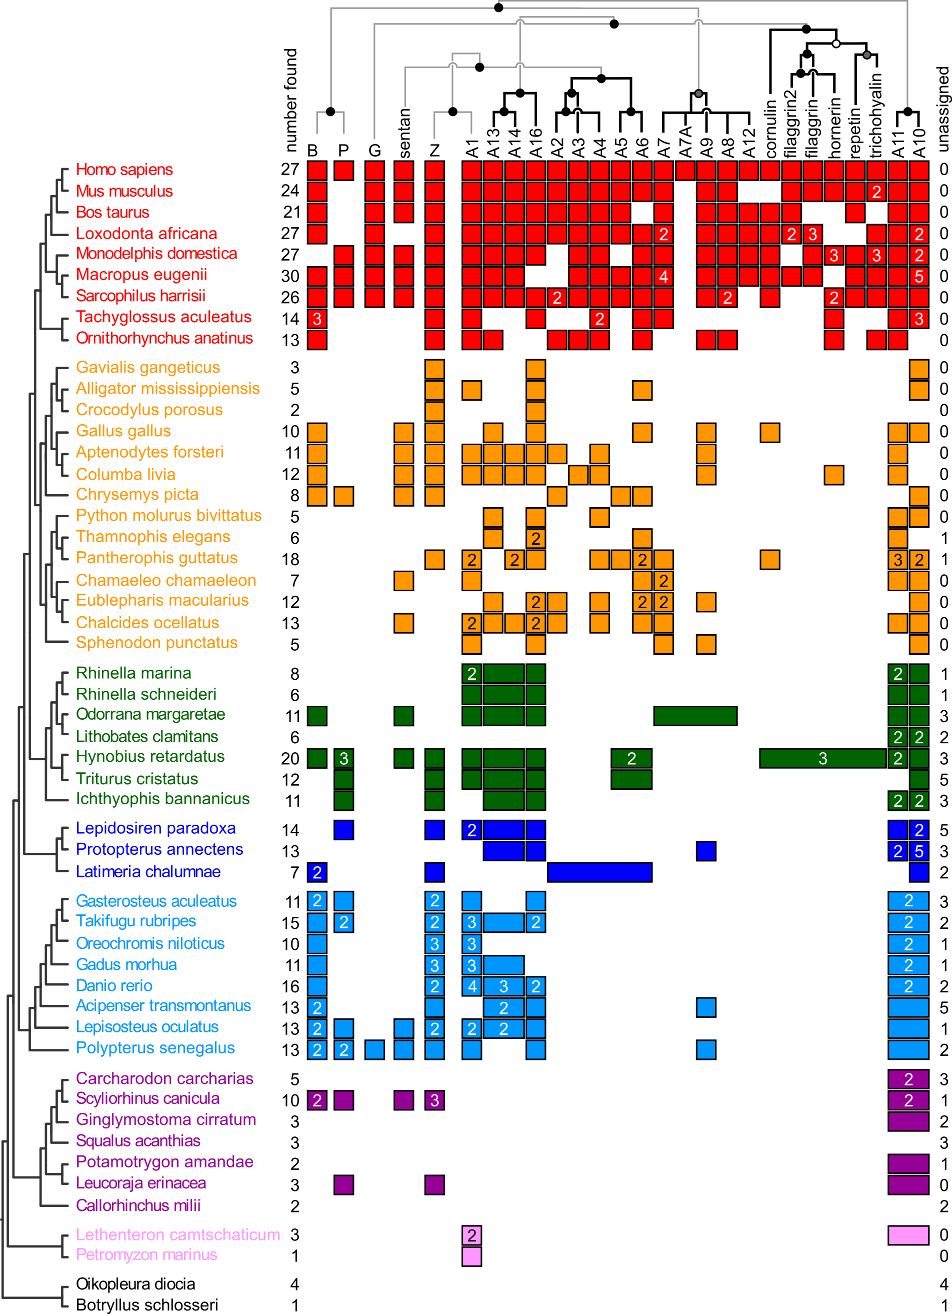
\includegraphics{ch3-fig3-smaller.png} 
\caption[Phylogeny, synteny, and taxonomic distribution provide a picture of S100 evolution]{Model-based phylogeny, synteny, and taxonomic distribution provide a consonant picture of S100 evolution. The human S100 orthologs are shown across the top, in the order they occur in the human genome. B, P, G, and Z occur on different chromosomes; A1-A10 are in a contiguous region of chromosome I. Sentan, an evolutionary relative, is also on a different chromosome. Species are shown on the left, organized by taxonomy. Color indicates taxonomic class, as in Fig 5. Squares denote the presence of an ortholog to the human gene for each species; a number in the box indicates the number of co-orthologous genes found in that species (if more than one); squares fused into a rectangle indicate a gene found in an earlier branching lineage that subsequently duplicated somewhere along the lineage leading to Homo sapiens. Total number of genes found for each species are shown on the left. The number of genes that were not orthologous to human genes (or could not be classified) are shown on right. Top tree shows the maximum-likelihood phylogeny of the family mapped onto the S100 genes found in the human genome. Circles denote SH support $\geq$ 0.85 (black); $\geq$ 0.75 (gray), $<$ 0.75 (white). Branches supported by both the ML phylogeny and synteny are shown in black; branches supported by only the ML tree are shown in gray.\label{samplefigure}}	
\end{figure}

There is strong correlation between the S100 subfamilies identified
in model-based phylogenetics and the distribution of the genes across
human chromosome I. Proteins with shared evolutionary relationships
form blocks across this region, suggesting local expansion by gene
duplication. The ML relationship between orthologs are shown above
the plot in Fig 6. The clades identified in our model-based phylogenetics
form individually contiguous blocks: A13-A16, A2-A6, A7-A12, S100-fused,
and A11-A10. This consonance between the phylogenetic signal and genomic
arrangement supports the shared ancestry of these subfamilies.

The species distribution of these orthologs then provides insight
into the diversification of the family. For example, A10, A11, or
their common ancestor (A10/A11) are found in all vertebrates, demonstrating
that this protein arose no later than the last common ancestor of
vertebrates. Because some genes may have been missed within each species\textemdash either
through lineage-specific loss or incomplete genomic/transcriptomic
coverage\textemdash this is a lower bound on the age of the gene.
After its origin, A10/A11 then diversified in later lineages. In the
bony fishes, A10 expanded, as reflected in the increased numbers of
genes co-orthologous to A10/A11. A10/A11 gave rise to the tetrapod
paralogs A10 and A11 via tandem gene duplication in the ancestor of
the lobe-finned fishes.

Another ancient S100 by this analysis is A1, which, intriguingly,
brackets the other end of the contiguous S100 genome region mammals
and some fishes \cite{shang_chromosomal_2008}. The simplest interpretation
of this pattern would be that the A1 or A10/A11 gene was the earliest
gene in this syntenic block, and that the remaining family arose by
serial expansion from that starting point.

Other ancient S100 orthologs are B, P, and Z. Our tree provides some
evidence that A1 and Z share a common ancestor, and that B and P share
a common ancestor. Intriguingly, these four ancient proteins are scattered
throughout vertebrate genomes, rather than being a part of the expanded
gene region containing A1-A10. This suggests that the last common
ancestor of jawed vertebrates had a collection of four to five S100
proteins, but that only the region containing A1-A10 then continued
to expand with the radiation of the vertebrates. Sentan\textemdash a
close evolutionary relative to the S100 family that does not possess
the diagnostic pseudo EF-hand of true family members\textemdash also
arose in the early vertebrates. Given the ambiguity of the deepest
branching of the tree, it is unclear whether it is an out group or,
instead, a duplication of an established S100 paralog.

The gene block containing A1-A10 expanded by what appears to be a
set of local gene duplication events. A13/A14 and A16 likely arose
next, at least by the ancestor of bony vetebrates. Like A10/A11, these
genes were duplicated through the whole genome duplications of teleost
fishes, giving rise to multiple S100 genes that are co-orthogolous
to the human genes in bony fishes. The tetrapod paralogs A13 and A14
did not arise until the amniotes, when they formed via duplication
from A13/A14. The next phase of expansion was local duplication that
led to the ancestors of A2-A6, A7-A12, and the S100-fused proteins
in early tetrapods. These founding genes then expanded across the
tetrapods, with several duplicates preserved in Sauropsids. The final
mammalian complement was achieved by several more duplications. The
A7-A12 and S100-fused clades\textemdash which are directly adjacent
in mammalian chromosomes\textemdash continue to rapidly expand by
duplication.

\subsection{Transition metal binding is nearly universal across the family}

With the phylogenetic tree in hand, we next set out to determine the
distribution of transition metal binding across the tree. Previously
reported transition metal binding is scattered across the tree (Fig
4, red proteins) \cite{moroz_role_2010,gilston_binding_2016}. If
this feature were ancestral, we predicted that transition metal binding
would be present across the majority of the tree. To test this hypothesis
we used isothermal titration calorimetry (ITC) to measure the ability
of human S100 proteins to bind to Zn$^{2+}$ and Cu$^{2+}$\textemdash the
two most prevalent transition metals encountered biologically\textemdash under
approximately physiological conditions (125 mM ionic strength, pH
7.4, 25$^{\circ}$C). We chose proteins that would maximize the sampling
across clades. Some of the proteins we selected have been reported
to bind transition metals, albeit with variable stoichiometry \cite{koch_implications_2007,tsvetkov_thermodynamics_2010}.
The other paralogs have, to our knowledge, yet to be characterized.

\begin{figure}
\centering
	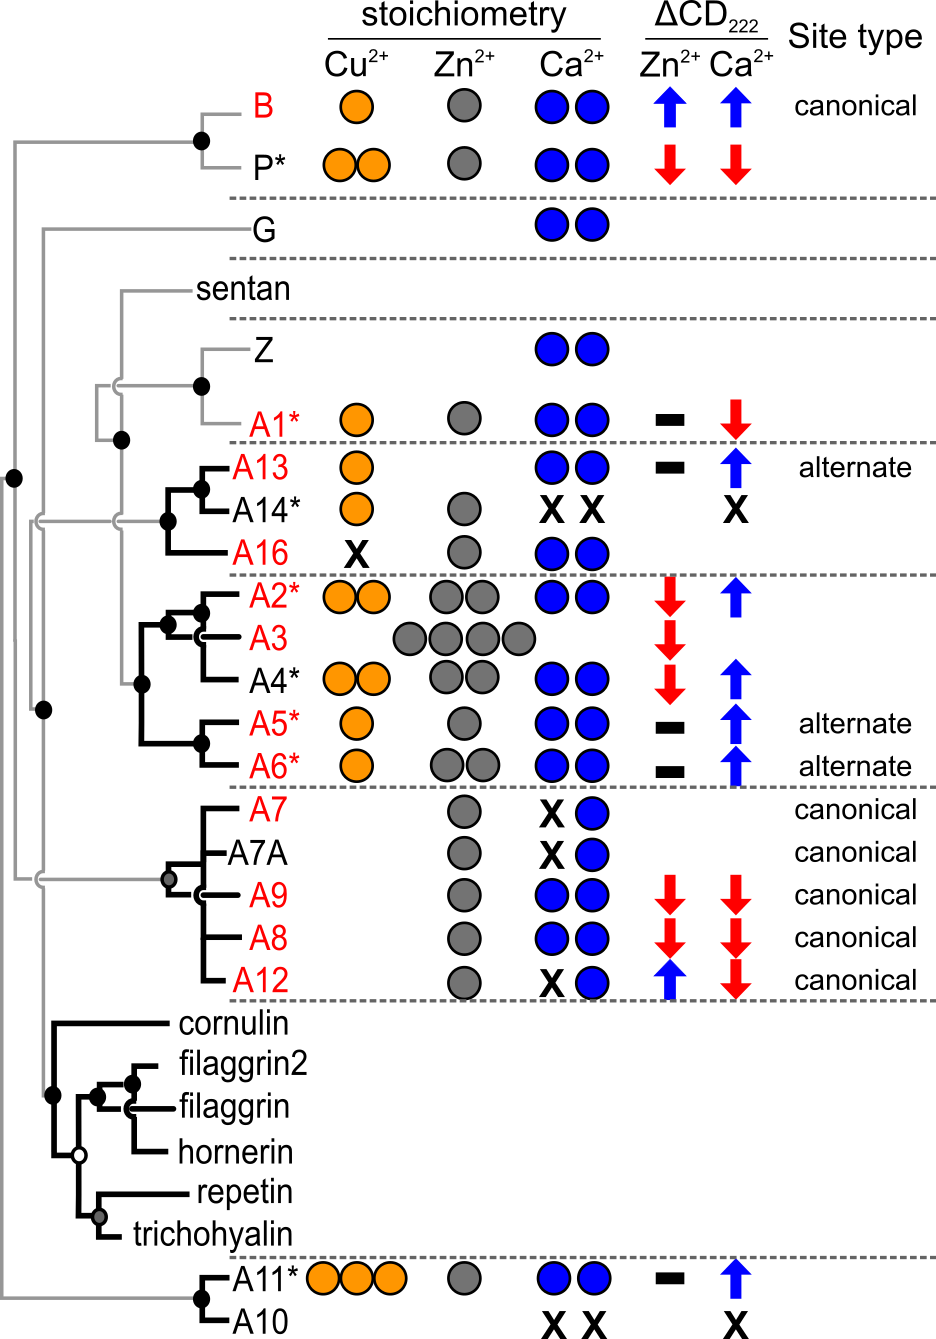
\includegraphics{ch3-fig4.png} 
\caption[Transition metal binding is conserved in the S100 family]{The human S100 paralogs are shown on the left, organized as on the top of Fig 6. Asterisks indicate S100 proteins investigated in the current study; red color indicates a protein for which transition metal binding has been noted in the literature previously. Biochemical properties of the human paralogs are shown as columns. Circles denote stoichiometry of binding for Cu$^{2+}$ (orange), Zn$^{2+}$ (gray), and Ca$^{2+}$ (blue). “X” indicates that the protein does not bind the metal; empty space is unmeasured. Arrows indicate the change in far-UV CD signal with the indicated metal: no change (black), increase (blue), and decrease (red). The transition metal binding site is indicated as “canonical” (B-like) or “alternate” (some other site).\label{samplefigure}}	
\end{figure}


We found that Zn$^{2+}$ and Cu$^{2+}$ binding was universally distributed
across the tree: every single S100 protein we characterized bound
to Zn$^{2+}$ and/or Cu$^{2+}$ with low micromolar affinity (Fig
4 and Fig 26 in supplement, S3 Table in supplementary directory) \cite{damo_molecular_2013,koch_implications_2007,vorum_expression_1996,kordowska_ca2+_1998,fritz_crystal_2002,schafer_brain_2000,baudier_ions_1986}.
With one exception, stoichiometry ranged from 1:1 to 3:1 (metal:monomer).
These binding affinities and stoichiometries are similar to previously
measured transition metal binding affinities for S100 proteins \cite{gilston_binding_2016,vorum_expression_1996,schafer_brain_2000,moroz_both_2009}.
Buffer-specific enthalpies ranged from -5.4 to 6.1 kcal/mol; the majority
of the enthalpies were negative. All of the proteins tested bound
to both Zn$^{2+}$ and Cu$^{2+}$, with the exception of A1 which
did not bind Cu$^{2+}$ under our experimental conditions. The Zn$^{2+}$
binding isotherm for A6 and the Cu$^{2+}$ binding isotherms for A2
and A4 were not well fit by standard binding models (as is often observed
for metal binding studies by ITC: \cite{wilcox_isothermal_2008}),
however, from the curves we could gain insight into their stoichiometry.
The A6/Zn$^{2+}$ and A4/Cu$^{2+}$ curves exhibited two phases, consistent
with two binding sites. The A2/Cu$^{2+}$ curve was quite broad, consistent
with $>$2 metals binding per monomer. Representative binding isotherms
for Zn$^{2+}$ and Cu$^{2+}$ to a variety of S100 proteins\textemdash including
the three problematic curves\textemdash are shown in Fig 26 in supplement. All measured
thermodynamic parameters are reported in S3 Table in supplementary directory.

We next asked if the structural response to these metals, like the
binding constant, was consistent across the tree. We measured Zn$^{2+}$-induced
changes in secondary structure by comparing the far-UV circular dichroism
(CD) spectra of these proteins with EDTA versus saturating Zn$^{2+}$
(Fig 27 in supplement). We found the response was variable across the family (Fig
4) \cite{koch_implications_2007,vorum_expression_1996,schafer_brain_2000,sturchler_s100a16_2006,becker_s100p_1992,rety_crystal_1999,wilder_location_2003,wright_three-dimensional_2005,garrett_biosensor_2008,murray_structural_2012,babini_structural_2011}.
For some proteins, Zn$^{2+}$ induced a decrease in CD signal (P,
A2 and A4); in others, it had no effect (A1, A11, A5 and A6). We also
observed Zn$^{2+}$-induced protein precipitation in the case of A14,
which was rapidly reversible by the addition of excess EDTA. We also
asked whether the structural response to Zn$^{2+}$ exhibited by these
proteins correlated with the response to their canonical agonist Ca$^{2+}$.
We found that they were largely uncorrelated (Fig 7 and Fig 27 in supplement). For
example, P has decreased CD signal with both Zn$^{2+}$ and Ca$^{2+}$,
while A2 shows decreased signal with Zn$^{2+}$ and increased signal
with Ca$^{2+}$.

When placed onto the phylogenetic tree, a few patterns in these responses
emerge (Fig 7). Phylogenetically close members of the family appear
to display similar structural responses to Zn$^{2+}$ binding. For
example, the closely related A2 and A4 proteins show qualitatively
similar decreases in CD signal in the presence of Zn$^{2+}$ relative
to the apo form. Likewise, the far-UV CD signal of direct sister proteins
A5 and A6 is insensitive to Zn$^{2+}$. This said, such patterns are
not universal. For example, B and P are directly sister but have opposite
structural responses to Zn$^{2+}$. Further, family members exhibit
all possible combinations of increased and decreased CD signal with
the addition of Ca$^{2+}$ and Zn$^{2+}$, revealing the variability
of this trait over evolutionary time.


\subsection{Early-diverging tunicate S100s bind transition metals}

Given that all human paralogs we characterized were capable of binding
transition metals, we predicted that this was a conserved, early feature
of the protein family. To test this prediction, we turned to two tunicate
homologs, which represent some of the earliest-diverging S100 proteins.
We selected two \textit{Oikopleura dioica} proteins\textemdash tunA
(tunicate A, CBY12809.1) and tunB (tunicate B, CBY30360.1)\textemdash for
characterization. Although the orthology of these proteins is unclear,
the proteins sample the breadth of tunicate S100 diversity, exhibiting
only 26.2\% identity. We expressed and purified these proteins, and
then characterized their metal binding features.

Because these proteins have not been characterized previously, we
first performed a baseline characterization to verify that they behave
like other S100 proteins. We first measured Ca$^{2+}$ binding. Like
many other S100 proteins, both tunA and tunB bound Ca$^{2+}$ with
nanomolar to micromolar dissociation constants and 2:1 (per monomer)
stoichiometry (Fig 8A and Fig 28 in supplement). Further, both proteins exhibited
changes in secondary and/or tertiary structure\textemdash as measured
by far-UV circular dichroism (CD) and intrinsic fluorescence\textemdash with
the addition of saturating amounts of Ca$^{2+}$ (Fig 8B and 5C and
Fig 28 in supplement). All of the observed changes were strictly metal dependent
and reversible upon the addition of EDTA. Metal-dependent changes
in conformation, as reflected in these changes in spectroscopic signals,
are a hallmark of S100 proteins \cite{koch_implications_2007,bertini_solution_2009,mani_circular_1983,schafer_s100_1996}.

\begin{figure}
\centering
	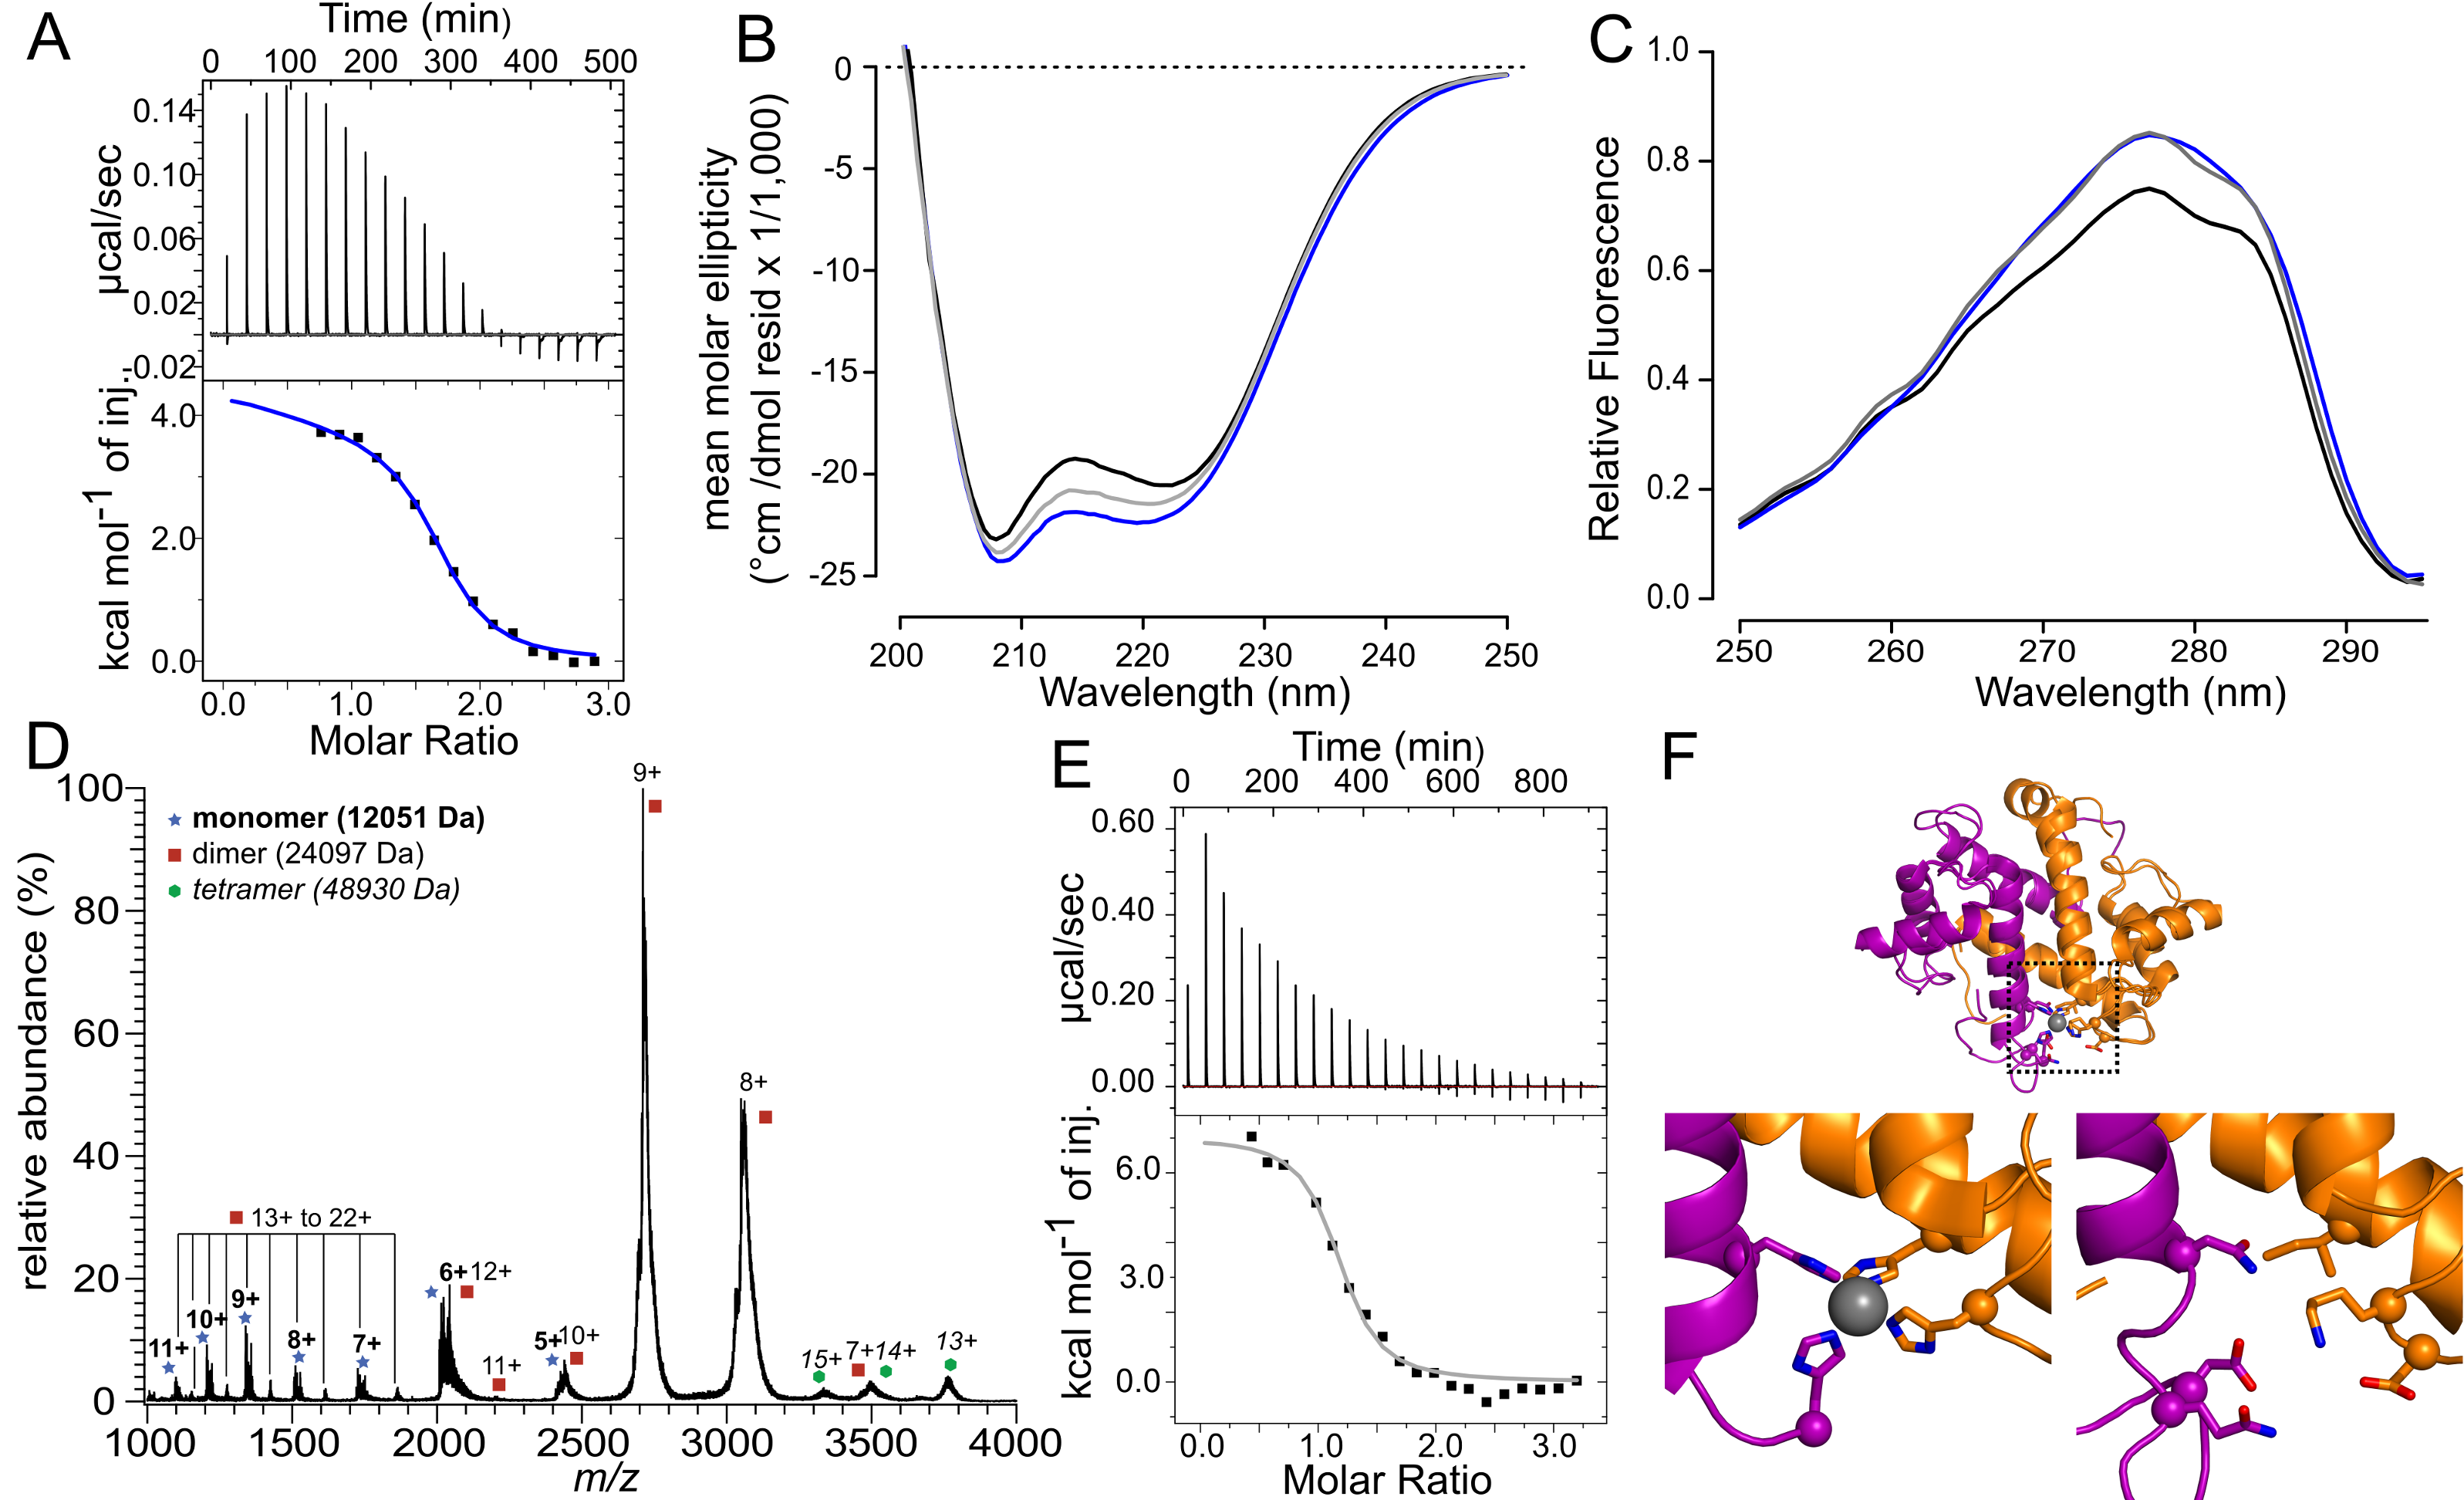
\includegraphics{ch3-fig5-smaller.png} 
\caption[Early-branching tunicate S100 binds transition metals at a non-canonical site]{Early-branching tunicate S100 binds transition metals at a non-canonical site. Colors indicate the metal present during experiment: Zn$^{2+}$ is gray, Ca$^{2+}$ is blue. A) Ca2+ binding to tunB by ITC. Top panel shows power traces for injections; bottom curve shows integrated heats and model fit to extract thermodynamic parameters. B) Far-UV circular dichroism spectra of the apo protein (black), Ca$^{2+}$ bound protein (blue), or Zn$^{2+}$ bound protein (gray). C) Intrinsic fluorescence spectra, with samples colored as in panel B. D) Mass spectrum of tunB. Notes above each peak indicate molecular weight and corresponding oligomeric state. E) Zn$^{2+}$ binding to tunB by ITC, with subpanels as in A. E) Homology model of tunB overlaid on crystal structure of human S100B (PBD: 3ZCT). Ligating residues are shown as sticks, with Cα atoms shown as spheres. A and B chains of the dimer are shown in orange and purple, respectively. Zn$^{2+}$ ion is shown as gray sphere. Top panel shows overlay, with box highlighting the zoomed-up regions shown at right. Bottom left panel shows S100B structure with Zn$^{2+}$ chelation. Bottom left panel shows tunB homology model, highlighting residues that would have to chelate Zn$^{2+}$.\label{samplefigure}}	
\end{figure}


We then assessed the ability of these proteins to form homodimers\textemdash a
key feature of most S100 proteins\textemdash using native electrospray-ionization
mass spectrometry (nanoESI) \cite{hernandez_determining_2007}. For
tunB, we detected homodimers (Fig 8D). The narrow distribution of
relatively low charge states observed in the nanoESI mass spectra
for both the monomer and dimer ions indicate that the proteins are
not denatured under these conditions and undergo little unfolding
during the ionization process. The broad mass spectral peaks observed
are the result of adduction of residual sodium from solution that
has survived buffer exchange. To see if the dimer peaks were the result
of non-specific aggregation during the electrospray process, we measured
dimerization at protein concentrations at which non-specific dimerization
is not expected ($<$ 1 $\mu$M, see methods). We found homodimers,
even at 10 nM protein, consistent with a specific tunB dimer (Fig 29 in supplement).
We also observed a small amount of homotetramer; however, the tetramer
was not robust to dilution and is likely an artifact of the electrospray
process (Fig 29 in supplement). For tunA, we detected homodimers; however, these
were not robust to dilution, suggesting that dimerization is relatively
weak for this protein (Fig 28 in supplement). We corroborated these observations
for tunA and tunB using a sedimentation velocity experiment (Fig 30 in supplement).
Under these conditions, we found that tunB was primarily a dimer.
In contrast, tunA exhibited both monomer and dimer species, consistent
with this protein forming a weaker dimer. Further work is required
to determine the precise distribution of oligomeric species in solution
for these proteins; however, these results are consistent with both
proteins having the ability to form homodimers, like other S100 proteins
\cite{streicher_modulation_2010}.

We next turned our attention to Zn$^{2+}$ binding. By ITC, both tunA
and tunB bound to Zn$^{2+}$ with nM to $\mu$M affinity and stoichiometries
of 2:1 (Fig 8E and Fig 28 in supplement). We attempted to verify these stoichiometries
by ESI-MS; however, we were unable to disentangle specific from non-specific
metal adduction in these samples. We then measured the changes in
secondary and tertiary structure measured by far-UV CD and intrinsic
tyrosine fluorescence. Although both proteins bound Zn$^{2+}$ tightly,
only tunB displayed a pronounced structural response, similar to that
induced by Ca$^{2+}$ binding (Figs 5B and 6C). The secondary structure
of tunA was insensitive to Zn$^{2+}$ binding although the protein
displayed a moderate increase in intrinsic tyrosine fluorescence (Fig 28 in supplement).

\begin{figure}
\centering
	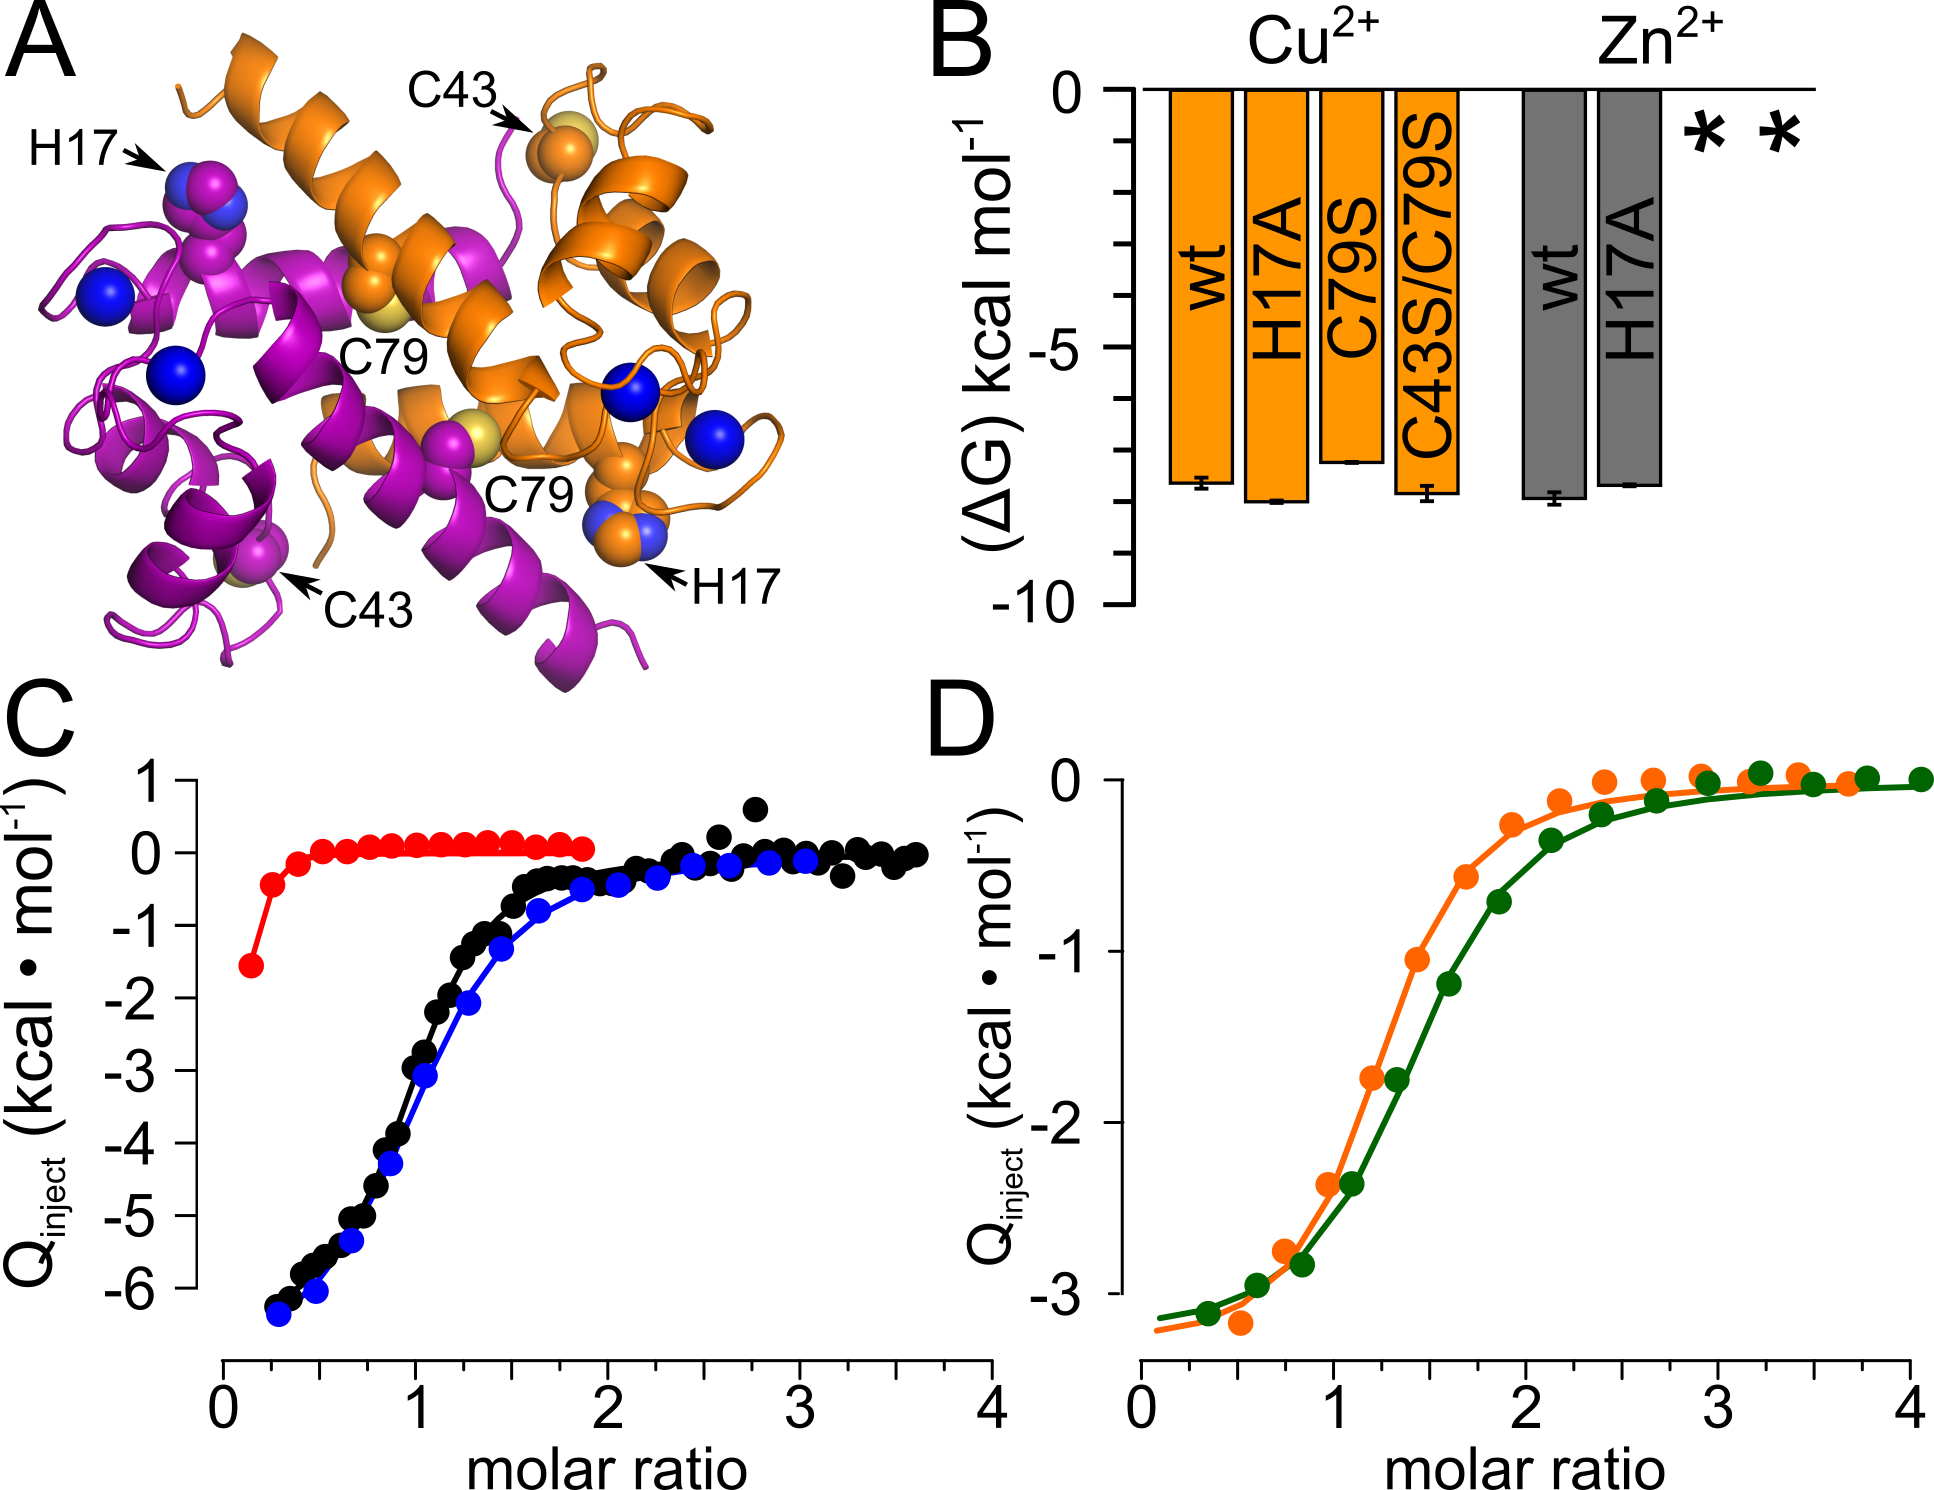
\includegraphics{ch3-fig6.png} 
\caption[Human S100A5 does not bind transition metals at the same site as B and the calgranulins]{Human S100A5 does not bind transition metals at the same site as B and the calgranulins. A) Mutated residues mapped onto the NMR structure of Ca$^{2+}$--bound human A5 (PDB: 2KAY). Dimer chains are colored purple and orange. H17, C43, C79 and Ca$^{2+}$ ions are shown as spheres. The location of H17 corresponds to the transition metal site in calgranulins and B (Fig 4B); C43 and C79 are in different regions of S100A5. C) Binding free energies measured for Cu$^{2+}$ (copper) and Zn$^{2+}$ (gray) to human A5 and its mutants. Zn$^{2+}$ binding constants could not be extracted for the C43S and C43S/C79S proteins (*). C) Integrated heats for ITC titration of Zn$^{2+}$ onto A5 (black), A5/H17A (blue) and A5/C43S (red). D) Integrated heats for ITC titration of Cu$^{2+}$ onto A5 in the absence (orange) or presence (green) of saturating (500 $\mu$M) Zn$^{2+}$.\label{samplefigure}}	
\end{figure}


\subsection{Transition metal binding occurs at independently evolved binding sites}

The broad distribution of transition metal binding across human paralogs,
along with the observed transition metal binding in the early-branching
tunicate proteins, suggests that transition metal binding is an essentially
universal property of this family. We next sought to understand to
what extent transition metal binding across the family reflects a
common binding site, or rather convergent acquisition of metal binding
on multiple lineages. Transition metal bind- ing to S100 proteins
has been extensively characterized in B and the \textquotedblleft calgranulin\textquotedblright{}
clade (A7,A8,A9,A12,A15), where it occurs at the same site, using
similar ligating residues (Fig 4B). B is an ancient protein, arising
at least as early as the cartilaginous fishes (Fig 6). In contrast,
the calgranulins arose $\sim$80 million years later in the ancestor
of amniotes (Fig 6). If the common site reflects shared ancestry,
we would expect to observe the same site across a wide variety of
descendants\textemdash possibly explaining the ubiquity of transition-metal
binding across the tree.

We first investigated the clade containing A2,A3,A4,A5, and A6. All
members of this clade possess a conserved histidine that, in B and
the calgranulins, coordinates transition metals (Fig 9A). We chose
to investigate human A5, as it binds to both Zn$^{2+}$ and Cu$^{2+}$
with 1:1 stoichiometry, and thus simplifies identification of the
binding site. We mutated His17 to Ala in human A5 and measured metal
binding of the mutant. Surprisingly the H17A mutation had only a small
effect on Zn$^{2+}$ binding (1.3 +/- 0.3 to 3.0 +/- 0.1 $\mu$M),
suggesting it is not directly involved in the binding of Zn$^{2+}$
in human A5. Additionally, this mutation did not compromise Cu$^{2+}$
binding (Fig 9B). Previous reports suggested that Cys residues in
the loop between helices 2 and 3, as well as those near the N and
C-termini, could play a role in binding divalent transition metals
in this clade \cite{moroz_role_2010,koch_implications_2007,kordowska_ca2+_1998}.
We therefore mutated these residues to serine in A5 and measured binding
of Zn$^{2+}$ and Cu$^{2+}$ to the mutants. Mutating the C-terminal
Cys (C79S) had no effect on Cu$^{2+}$ binding, but led to a drastic
change in the Zn$^{2+}$ binding curve (Fig 9C). The apparent stoichiometry
of binding was drastically reduced ($\sim$0.1), which is consistent
with only a small fraction of the protein being competent to bind
Zn$^{2+}$. Additionally, the enthalpy of binding is mostly ablated.
These results clearly indicate that C79 is involved in Zn$^{2+}$,
but not Cu$^{2+}$ binding. We attempted to ablate Cu$^{2+}$ binding
by also mutating the loop Cys residue (C43S), but found that this
double Cys mutant (C43S/C79S) still left Cu$^{2+}$ binding unaffected
(Fig 9B). These results show that Zn$^{2+}$ and Cu$^{2+}$ not only
bind outside the B/calgranulin site, but bind at different sites on
the same protein. To confirm that these metals bind at different sites,
we also measured binding of Cu$^{2+}$ to Zn$^{2+}$-saturated human
A5 and found no evidence of competition between the two metals (Fig
6D). Finally, because mutating H17, C43, and C79 did not disrupt Cu$^{2+}$
binding, we hypothesized that the metal might bind at one of the Ca$^{2+}$
binding motifs. We therefore repeated the Cu$^{2+}$ binding curve
in the presence of saturating (2 mM) Ca$^{2+}$. We observed extensive
aggregation, however, which made interpretation of the ITC binding
isotherm impossible. This suggests that previously-noted antagonism
between Ca$^{2+}$ and Cu$^{2+}$ \cite{schafer_brain_2000} may be
an artifact of aggregation rather than true antagonism.

We next turned our attention to the tunicate protein tunB. This protein
behaves like a conventional S100 protein, forming a homodimer, binding
to Ca$^{2+}$ and changing its structure in response to metals (Fig
5A\textendash 5E). Further, it binds to transition metals with a 2:1
stoichiometry. To determine if it could bind metals at the canonical
transition metal binding site, we constructed a homology model for
the protein and then inspected the residues that would form the S100B/calgranulin
binding pocket. These are Asp, Gln, Asn, and Lys (Fig 8F). The lack
of a His or Cys residue suggests this site is not capable of binding
transition metals. Thus, transition metal binding in this early-branching
ortholog almost certainly occurs at a different site.


\section{Discussion}

Our work provides a high-level view of the evolution of the S100 protein
family and the ability of its members to bind to divalent transition
metals. Our work provides the best-resolved phylogeny yet determined
for this family. All characterized human paralogs, as well as two
early-branching tunicate S100 homologs, bind to transition metals
with a physiologically relevant $\sim$$\mu$M binding constant. On
the other hand, different S100 proteins bind at different transition
metal binding sites. Thus, the apparently \textquotedblleft conserved\textquotedblright{}
feature of transition metal binding actually reflects independent
acquisition of metal binding on multiple lineages. Further, the structural
changes induced by transition metal binding are variable, suggesting
quite different mechanisms of binding and possible functional consequences
for different family members.


\subsection{Transition metal binding occurs at independently evolved binding sites}

Our work, combined with previous publications, reveals at least four
sites\textemdash and therefore four evolutionary origins\textemdash of
transition metal binding in the S100 family: the B/calgranulin site
(Fig 4B), A5's Cys-79 site (Fig 9), an N-terminal Cys in A2 \cite{koch_implications_2007},
and a unique glutamate-rich site in human A13 \cite{arnesano_structural_2005}.
The plasticity of this feature is likely because of the relative ease,
biochemically, of creating transition metal binding sites \cite{yamashita_where_1990,babor_prediction_2008,rubino_coordination_2012}.
A few amino acid substitutions can create a new site, while a few
other substitutions ablate an existing site. This is similar to the
evolutionary behavior of phosphorylation sites, which can shift rapidly
over evolutionary time \cite{holt_global_2009}. Additionally, some
of the proteins may bind to transition metals in one of the Ca$^{2+}$
binding motifs of an S100. For example, Gribenko et al. proposed that
human S100P may bind Zn$^{2+}$ in one of the Ca$^{2+}$ binding motifs
\cite{gribenko_oligomerization_1998}. EF-hands often discriminate
Ca$^{2+}$ from Zn$^{2+}$ and Cu$^{2+}$, however, so this likely
does not explain all of the observed transition metal binding \cite{arnesano_structural_2005,mills_metal_1985,grabarek_insights_2011,chung_ef-hand_2016}.

Another feature of Zn$^{2+}$ and Cu$^{2+}$ binding in this family
is that of variable structural responses to the same metal. Even closely
related S100 proteins undergo different conformational changes when
bound to a transition metal (Fig 7). This likely allows different
orthologs to play different functional roles in response to transition
metal binding. This can be seen for proteins that have been studied
in detail. For example, human A13, which binds Cu$^{2+}$ at a unique
site, has been proposed to be involved in chaperoning Cu$^{2+}$ as
part of FGF release \cite{sivaraja_copper_2006}. A9 provides another
example of diverse responses to transition metals. When A9 is alone,
Zn$^{2+}$ binding is strictly necessary for one function (TLR4-activation)
\cite{bjork_identification_2009}, but strongly inhibits another function
(arachidnoic acid binding) \cite{kerkhoff_zinc_1999}. This site is
modified in vivo through the formation of a heterodimer with A8, which
changes the ligating residues for one half of the site \cite{damo_molecular_2013,gagnon_manganese_2015}.
This creates an extremely high affinity site for Mn$^{2+}$ and Zn$^{2+}$
that inhibits bacterial growth by starving them of these metals \cite{damo_molecular_2013}.

Much of the transition metal binding we have observed plays no known
role, but the observed binding constants ($\sim$$\mu$M) are consistent
with biological concentrations of divalent transition metals. In particular,
many S100 proteins are found in the extracellular space \cite{donato_intracellular_2003},
where Zn$^{2+}$ concentrations can be high enough to occupy these
sites \cite{hopt_methods_2003,hyun_zinc_2004}. We expect further
roles of transition metal binding to be identified in this family
as it is further characterized \cite{moroz_role_2010,gilston_binding_2016}.

\subsection{Expansion of the family}

In addition to providing insight into the evolution of transition
metal binding, our phylogenetic analysis provides insight into the
overall pattern of expansion of the S100 protein family. Previous
phylogenies used highly incomplete taxonomic sampling and, with the
exception of \cite{kraemer_structural_2008}, distance-based phylogenetics
\cite{zimmer_evolution_2013,marenholz_s100_2004,shang_chromosomal_2008}.
We used many more sequences, from many more taxa, and applied a combined
model-based/synteny analysis to better disentangle the history of
the family. Our work provides support for evolutionary relationships
between A13-A16, A2-A6, the calgranulins, the S100-fused proteins,
and A10/A11 despite the relatively weak support for these clades taken
from a purely model-based phylogenetic perspective. This also supports
the previously proposed model of local gene duplication \cite{zimmer_evolution_2013,marenholz_s100_2004,shang_chromosomal_2008}.

Our work provides evidence for earlier origins of many S100 family
members than previously reported. For example, we found that the S100A2-A6
clade likely arose in ancestor of all tetrapods, and that it had the
complete mammalian complement by the ancestor of amniotes. In contrast,
Zimmer et al proposed this clade arose in the ancestor of mammals
\cite{zimmer_evolution_2013}. Some orthologs (A1, B, P, and Z) have
likely been present since the last-common ancestor of vertebrates.
Further, we expect that many S100 proteins actually arose even earlier
than our analysis suggests. Despite having broader sampling than previous
studies, our sampling of tunicates, jawless fishes, and cartilaginous
fishes was still relatively sparse. Further, we relied heavily on
transcriptomes, which likely underestimate the S100 complements for
these organisms. As more genomic and transcriptomic datasets for these
species become available, we expect to observe even earlier origins
of many of the mammalian S100 orthologs.

Another difference between our tree and the published tree by Kraemer
et al. \cite{kraemer_structural_2008} is that we do not see radical,
parallel expansion of the S100s in bony fishes. Rather, most S100
proteins from the bony fishes are orthologous to mammalian S100s.
For example, we identified 15 S100 proteins in Takifugu rubripes (pufferfish).
All but two of them could be assigned as orthologs to human proteins
(Fig 6). This said, many of these do represent lineage-specific duplications\textemdash likely
via the whole genome duplications that have occurred in teleost fishes\textemdash that
are co-orthologous to human proteins. The difference between our results
and the previous phylogeny likely arises from our much broader sequence
sampling, as the Kraemer et al. dataset was strongly biased towards
sequences taken from teleosts \cite{kraemer_structural_2008}.

Despite extensive taxonomic sampling, the phylogenetic tree we report
is not fully resolved: the deepest branches remain obscure. This is
because of the large amount of sequence divergence that has occurred
between many S100 protein family members, their relatively short sequences,
and the number of orthologs make full resolution of this family quite
challenging. Resolution can likely be increased for individual subfamilies
within the tree through even denser sampling. For example, adding
further aminotes may help resolve the relationships between the amniote-specific
clades identified in our analysis. We also believe increasing the
sampling of amphibians would be particularly powerful, as we relied
heavily on amphibian transcriptomes and likely missed S100 proteins.
Better characterization of S100 proteins from amphibians may help
disentangle the origins and relationships of some of the tetrapod-specific
S100s (such as the calgranulins) which are, as yet, difficult to resolve.
Further, signal for these relatively recent proteins could be boosted
by using codon rather than amino acid substitution models.

\section{Conclusion}

Our work reveals that transition metal binding is both ubiquitous
and evolutionarily labile within the S100 protein family. Many have
noted that much of the diversity of S100 function is determined by
altered expression of family members \cite{marenholz_s100_2004,bertini_solution_2009,h_differential_1987,zimmer_tissue_1987,kuznicki_tissue_1989,zimmer_s100_1995,gribenko_molecular_2001};
however, our work highlights that these regulatory changes have also
been accompanied by changes in sequence and biochemistry. In particular,
the ease of creating and destroying transition metal binding sites
has allowed rapid changes in this feature of S100 proteins. As a result,
new metal binding behavior can be exploited to achieve functional
diversity in the family \cite{moroz_role_2010,gilston_binding_2016},
even while Ca$^{2+}$ binding and its induced structural changes remain
relatively conserved (Fig 7).

This biochemical diversification occurred rapidly during the expansion
of the S100 proteins, which are a relatively young protein family.
The details of how this diversification occurred are likely to encompass
a rich evolutionary story. As new S100s arose via gene duplication,
were they required to maintain metal binding while continuing to evolve?
Or, have there been multiple cycles of loss and subsequent regain
over the course of S100 evolution? What was the exact nature of metal-binding
in the last common ancestor of all S100 proteins? Our observations
provide groundwork to begin to ask these questions.

\section{Materials and Methods}

\subsection{Sequence Set}

We generated a database of 564 S100 protein sequences, sampled from
52 chordate species, with an emphasis on even taxonomic sampling (S1
Spreadsheet). Previous publications and preliminary database searches
revealed S100 proteins were restricted to the chordates, \cite{zimmer_evolution_2013,marenholz_s100_2004,kraemer_structural_2008}
so we selected specific chordate species and characterized their S100
protein complements through extensive BLAST searches \cite{altschul_basic_1990}.
We used human proteins as seed sequences (including sentan and the
S100-fused proteins, S1 Table in supplementary directory). No published genome or transcriptome
data were available for some species, so we generated de novo transcriptomes
from RNAseq data in the short reads archive \cite{leinonen_sequence_2011}
using Trinity with default parameters \cite{grabherr_trinity:_2011}.
The sources for our analysis are shown in S2 Table in supplementary directory.

We removed duplicate sequences ($>$95\% identity) from within each
species using cdhit \cite{li_clustering_2001}, and removed sequences
less than 45 amino acids long. We then reverse BLAST'd all remaining
sequences against the human proteome to verify they encoded S100 proteins.
We aligned the sequences using msaprobs \cite{liu_msaprobs:_2010}
followed by manual refinement in aliview \cite{larsson_aliview:_2014}.
Refinement was minimal and consisted of truncating variable N-terminal
and C-terminal extensions, as well as several ambiguous indels. (We
truncated the fused S100 protein sequences to 150 amino acids covering
the S100 domain prior to alignment). The final alignment was 132 columns
and had robustly aligned key columns (Fig 24 in supplement and S2 Fig in supplementary directory, S1 Alignment in supplementary directory).


\subsection{Phylogenetic Trees}

We generated the ML tree using phyml \cite{guindon_new_2010} with
SPR moves starting from the neighbor-joining tree. 10 random starting
trees did not yield a higher likelihood tree. We found LG+Γ8 was
the highest likelihood model \cite{le_improved_2008}. We calculated
aLRT-SH supports for each node \cite{anisimova_survey_2011}. In pilot
analyses, the tunicate sequences were placed in random and unpredictable
places on the tree (for example, coming out with mammals or in other
nonsensical places on the tree). We therefore excluded them from the
final ML analysis (S1 Tree in supplementary directory).

We generated a Bayesian phylogenetic tree using Exabayes \cite{aberer_exabayes:_2014}.
We ran two replicate MCMC runs starting from different random trees,
each consisting of one main and three heated chains. We stopped the
runs after 10 million generations, giving a final average split frequency
of 3.97\% and log likelihood ESS of 3,315. We sampled substitution
models in addition to trees, giving a final 99.8\% posterior probability
for the JTT model \cite{jones_rapid_1992}. We used uniform priors
for all parameters. We discarded the first 15\% of the trees as burn-in
and generated a consensus tree by majority-rule, collapsing all nodes
with posterior probabilities $<$50\% (S2 Tree).

\subsection{Molecular cloning and Protein Expression/Purification}

S100 proteins were expressed from synthesized genes in a pET28/30
vector that had an N-terminal, TEV-cleavable His tag (Millipore).
Proteins were expressed in Rosetta (DE3) pLysS E. coli cells (Millipore).
A saturated overnight culture was used to inoculate 1.5 L cultures
at 1:150 ratio. Bacteria were grown to log-phase (OD600 $\sim$ 0.8\textendash 1.0)
shaking at 37$^{\circ}$C, followed by induction of protein expression
in 1 mM IPTG for $\sim$16 hr at 16$^{\circ}$C. Cells were harvested
by centrifugation. Pellets were frozen at -20$^{\circ}$C, where they
were stored for up to 2 months. Cells were lysed by sonication in
25mM Tris, 100mM NaCl, 25mM imidazole, pH 7.4.

Primary purification was done with a 5 mL HiTrap Ni-affinity column
(GE Health Science) on an $\ddot{A}$kta PrimePlus FPLC (GE Health
Science), using a 25mL gradient between 25 and 500 mM imidazole. Pooled
fractions were then incubated overnight at 4$^{\circ}$C in the presence
of $\sim$1:5 TEV protease. This cleaves the His-tag from the protein,
leaving the amino acids Ser-Asn in front of the wildtype starting
methionine. Proteins were further purified by hydrophobic interaction
chromatography (HIC) using a 5 mL HiTrap phenyl-sepharose column (GE
Health Science). This step takes advantage of the Ca$^{2+}$-dependent
exposure of a hydrophobic binding surface on the S100 proteins. Proteins
were equilibrated with 2 mM CaCl$_{2}$ and loaded onto the HIC column,
followed by a 30mL gradient elution in 25mM Tris, 100mM NaCl, 5mM
EDTA, pH 7.4. Proteins were then dialyzed into 4 L of 25 mM Tris,
100 mM NaCl, pH 7.4 buffer overnight at 4$^{\circ}$C. To remove the
small amount of uncleaved His-tagged protein present, proteins were
then passed over another 5 mL HiTrap Ni-affinity column and the flow
through collected. Finally, if any protein contaminants remained by
SDS-PAGE, we performed a final anion chromatography step using a 5mL
HiTrap DEAE column (GE), 25mM Tris, pH 7.0\textendash 8.5 (depending
on protein) buffer with a 50mL gradient to 500 mM NaCl.

Purified proteins were dialyzed overnight against 2L of 25mM TES (or
Tris), 100mM NaCl, pH 7.4, containing 2 g Chelex-100 resin (BioRad)
to remove divalent metals. Purity of final protein products were $>$95\%
by SDS PAGE and MALDI-TOF mass spectrometry. Final protein products
were flash frozen, dropwise, in liquid nitrogen and stored at -80$^{\circ}$C.
Typical protein yields were $\sim$20mg/L of culture.

\subsection{Protein characterization}

Prior to all biophysical measurements, we thawed and exchanged all
proteins into an appropriate buffer by two serial NAP-25 desalting
columns (GE Health Science). We then used A280 to determine protein
concentration using an empirical extinction coefficient for each protein.
To determine extinction coefficients, we first used ProtParam \cite{gill_calculation_1989,walker_proteomics_2005}
to calculate the extinction coefficient for each protein in 6 M GdmHCl
($\varepsilon$6MGdm). We then measured the difference in A280 for
an identical concentration of protein in native buffer versus in 6
M GdmHCl. We could then estimate a native extinction coefficient using
the relationship  $\varepsilon_{native}=\varepsilon_{6MGdm}\cdot A_{280,native}/A_{280,6MGdm}$.
For some proteins no correction from the predicted extinction coefficient
was necessary. Extinction coefficients used for calculation of protein
concentration are as follows: (hA5: 5540 M$^{-1}$cm$^{-1}$, hA6:5434
M$^{-1}$cm$^{-1}$, tunA:1490 M$^{-1}$cm$^{-1}$, tunB: 5699 M$^{-1}$cm$^{-1}$,
hA2:3230 M$^{-1}$cm$^{-1}$, hA4:3230 M$^{-1}$cm$^{-1}$, hA14:7115
M$^{-1}$cm$^{-1}$, hA1:8480 M$^{-1}$cm$^{-1}$, hA11:4595 M$^{-1}$cm$^{-1}$,
hP:2980 M$^{-1}$cm$^{-1}$). We also corrected for scatter in all
A280 measurements \cite{birdsall_correction_1983}.


We performed ITC experiments in 25 mM buffer, 100mM NaCl at pH 7.4
that had been chelex-treated and filtered at 0.22 $\mu$m. We selected
Tris or TES as the buffering species on a case-by-case basis to ensure
observable heats of binding. We equilibrated and simultaneously degassed,
either by application of vacuum to the solution or by centrifugation
at 18,000 $\times$ g at the experimental temperature for 60 minutes.
We dissolved metals (CaCl$_{2}$, ZnCl$_{2}$, or CuCl$_{2}$) directly
into the experimental buffer immediately prior to each experiment.
We performed all experiments at 25$^{\circ}$C using a MicroCal ITC-200
or a MicroCal VP-ITC (GE Health Sciences). Data were collected using
low gain or no gain, with 750 rpm syringe stir speed. Shot spacing
ranged from 120s-2400s depending on gain settings and relaxation time
of the binding process. These setting were optimized on a per protein
basis. Data were fit to one or two site models using the Origin 7
software. For binding curves with obvious 1:1 stoichiometry the one-site
model in Origin was used. For data with apparent 2:1 stoichiometry,
evident from location of inflection points in the data, a fit of the
included two-site model was attempted. If the two-site model could
not be fit, we then used a single-site binding model with a floating
stoichiometry to extract an apparent binding constant across sites.

We collected far-UV circular dichroism data between 200\textendash 250
nm using a J-815 CD spectrometer (Jasco) with a 1 mm quartz spectrophotometer
cell (Starna Cells, Inc. Catalog No. 1-Q-1). We prepared 20\textendash 50
$\mu$M samples in a TES buffer identical to that used for ITC. We
centrifuged at 18,000 x g in a temperature-controlled centrifuge at
the experimental temperature prior to experiments. We collected 5
scans for each condition, and then averaged the spectra and subtracted
a blank buffer spectrum using the Jasco spectra analysis software
suite. We converted raw ellipticity into mean molar ellipticity using
the concentration and number of residues in each protein. We collected
intrinsic tyrosine and/or tryptophan fluorescence using a J-815 CD
spectrometer (Jasco) with an attached model FDT-455 fluorescence detector
(Jasco) using a 1 cm quartz cuvette (Starna Cells, Inc.). We prepared
5\textendash 20 $\mu$M samples exactly as we did for our CD experiments.
We collected 3\textendash 5 replicate scans for each condition, and
then averaged the spectra and subtracted a blank buffer spectrum (averaged
from 10\textendash 15 buffer blank spectra) using the Jasco spectra
analysis software suite. For all spectroscopic measurements, we verified
the reversibility of metal-induced changes to the spectra by measuring
the apo spectrum, adding the appropriate metal and re-measuring the
spectrum, and then adding excess EDTA and re-measuring the spectrum.

\subsection{Native electrospray ionization time-of-flight mass spectrometry (nano ESI-MS)}

To prepare samples for mass spectrometry experiments small ($\sim$200$\mu$L) samples of the proteins used in MS experiments were dialyzed for at least 24 hr against 2--4 L of either 10 or 100mM ammonium acetate, pH 7.4 to remove salt and exchange into a more optimal buffer for MS. Samples were then diluted to $\sim$10$\mu$M in the dialysis buffer prior to experiment. All mass spectra were acquired using a Waters Synapt G2-Si ion-mobility mass spectrometer equipped with a nanoelectrospray (nanoESI) source and operated in “Sensitivity” mode. NanoESI emitters were pulled from borosilicate capillaries (ID 0.78 mm) to a tip ID of approximately 1$\mu$m using a Sutter Flaming-Brown P-97 micropipette puller. 3--5$\mu$L of sample were loaded into an emitter, a platinum wire was placed in electrical contact with the solution, and a potential of +0.8--1.2 kV was applied to the wire to initiate electrospray. The source temperature was equilibrated to ambient temperature, trap and transfer collision voltages were set to 25 V and 5 V, respectively, and the trap gas used was argon at a flow rate of 5 mL/min. Reported spectra are the sum of $\sim$3 minutes of continuously-collected data. Mass calibration was achieved using the series of Cs(CsI)$_{n}$$^{1+}$ peaks produced from nanoESI of 0.1 M aqueous cesium iodide (Aldrich).

We carefully controlled for spurious dimers in our nanoESI-MS experiments. Non-specific dimers (and high-order oligomers) can arise if, by chance, more than one monomer ends up in an electrospray drop. These non-specific aggregates are expected to follow a roughly Poisson distribution of oligomeric states, governed by the bulk concentration of monomers in solution. These non-specific species can be distinguished from specific oligomeric species by measuring the mass spectrum over a wide range of protein concentrations. Dimers observed at 10 $\mu$M could be the result of non-specific interactions; dimers observed at 10 nM are almost certainly not. This can be seen by considering the distribution of non-specific species across drops. Under our instrumental conditions, electrospray creates drops $\sim$100--200 nm in diameter, meaning that 10 nM protein solution will yield drops that contain, on average, $\sim$0.003--0.025 protein molecules. Taking the upper limit of 0.025 protein molecules per drop, one would expect only 0.2\% of drops to have non-specific dimers. Increasing to 100 nM protein takes this to 2.4\% of drops. If one goes to 1 $\mu$M, non-specific dimers become quite significant (25.6\%), but this is accompanied by a large number of non-specific trimers (21.4\%). Although many factors, including relative ionization efficiency and instrumental conditions, can affect the observed abundances of ions formed from electrospray, these effects should be largely independent of initial solution concentration under the instrumental conditions used here.

We interpreted the mass spectra shown in Fig 8D and S14 using this logic. Mass spectra of proteins at low concentrations (10--100 nM) exhibit unexpectedly abundant monomers and dimers, consistent with a specific dimer. Mass spectra at high concentrations (1--10$\mu$M) exhibit dimers but not trimers, again consistent with a specific dimer rather than non-specific, Poisson-governed aggregation in drops. The small population of tetramer for tunB at 10 $\mu$M could either reflect a true tetramer or a random partitioning of two dimers into an electrospray drop at this high concentration.

\subsection{Sedimentation velocity analytical ultracentrifugation}

Samples were concentrated to $\sim$50$\mu$M and then dialyzed against
2L of 25 mM TES, 100mM NaCl, 1mM TCEP, pH 7.4) overnight at 4$^{\circ}$C
using 6000\textendash 80000 MWCO dialysis tubing. Prior to sedimentation
velocity experiments proteins were then centrifuged at $>$18000 $\times$
g for 30 min. in a temperature-controlled centrifuge. AUC experiments
were performed at 50k x g in sector-shaped cells with sapphire windows
(Beckman) on a Beckman ProteomeLab XL-1 analytical ultracentrifuge.
Due to the low extinction coefficients of the proteins, sedimentation
was monitored using interference mode rather than absorbance at 280nm.
Sedimentation velocity data was fit numerically to the Lamm equation
and the c(s) distribution determined using SedFit \cite{schuck_size-distribution_2000,brown_macromolecular_2006}.
Estimated sedimentation coefficients and molecular masses of species
present in solution were calculated from the fits.

\subsection{Homology model}

The homology model of tunB was constructed using Modeller 9.17 \cite{webb_comparative_2002}
using 46 Ca$^{2+}$ bound crystal structures (without bound peptide
targets) as combined template(PDB:1e8a, 1gqm, 1j55, 1k96, 1k9k, 1mho,
1mr8, 1odb, 1qlk, 1xk4, 1xyd, 1yut, 1yuu, 1zfs, 2egd, 2h2k, 2h61,
2k7o, 2kay, 2l51, 2psr, 2q91, 2wnd, 2wor, 2wos, 2y5i, 3c1v, 3cga,
3cr2, 3cr4, 3cr5, 3czt, 3d0y, 3d10, 3gk1, 3gk2, 3gk4, 3hcm, 3icb,
3iqo, 3lk0, 3lk1, 3lle, 3m0w, 3psr, 3rlz, and 4duq). Alignment was
generated using the PAIRWISE alignment method with default parameters.
Model was generated as a dimer, with the single tunicate sequence
mapped to both the A and B chains. Automodel was used to generate
models, using default parameters. 20 models were generated and the
best selected by DOPE score. The final model had an RMSD of 0.65 $\mathring{A}^{2}$
relative to the crystal structure of S100B bound to Ca$^{2+}$ and
Zn$^{2+}$ (PDB: 3czt).


\section{Bridge to Chapter IV}


In this chapter, the phylogenetic tree of the S100 protein family was reconstructed. Subsequently, the binding of transition metal ions to the proteins was mapped onto the phylogeny by using a large set of human paralogs as representative clade members. Some data were already available in the literature and these were incorporated into the analysis. The results indicated that binding of transition metal ions is an almost universally-conserved feature of the S100 family. However, binding stoichiometry, metal-driven conformational changes, binding site ligands, and binding site location varied across the family. It was thus concluded that binding of transition metals is a conserved feature of S100s at the level of activity, but has diversified extensively at the biochemical level. Two early-branching S100 proteins from the tunicate \textit{Oikopleura dioica} were also characterized for the first time. These proteins displayed all the hallmark biochemical features of the more well-studied S100 proteins from higher metazoans: homodimerization, calcium-binding, transition metal binding, and metal-ion driven conformational changes. These results indicate that these canonical biochemical features of the S100s are ancestral to the family. This chapter highlights the striking evolutionary lability of an overall conserved biochemical feature, which has broader implications for understanding the evolutionary meanderings of protein traits. Chapter IV delves deeper into the biochemistry of metal binding in a specific member of the S100 protein family. S100A5 is a calcium binding protein found in a small subset of human tissues. Little is known about the biological roles of S100A5. Previous work indicated that S100A5 displays antagonism between binding of Ca2+ and Cu2+ ions, which is one of the most commonly cited features of the protein. The interplay between Ca2+ and Cu2+ binding by S100A5 is further characterized in this chapter. It is shown that S100A5 can actually bind to both Ca2+ and Cu2+ simultaneously without antagonism. Furthermore, it is demonstrated that the apparent antagonism observed in previous studies is likely due to aggregation of the protein induced by binding of metals. This chapter highlights further the diversity of biochemical modifications found in the S100 family and provides important data on S100A5 that will be useful for other researchers trying to understand it's biological functions. 
